\chapter{Auswertung}
\label{chap:Auswertung}
In diesem Kapitel sollen die im Experiment gewonnen Messdaten ausgewertet werden. Bereits bei einer Kalibrationsmessreihe mit Argon konnten aufgrund einer Fehlfunktion der Elektronenkanone keine vollständigen Wirkungsquerschnitte aufgenommen werden. Die Zahl der Elektronen, die für die Berechnung des Wirkungsquerschnittes benötigt werden, kann nicht ausreichend genau eingestellt werden, sodass gerade bei geringeren Energien keine Messung möglich ist. Nach einer Reperatur sollte dies wieder möglich sein. 

Aus diesem Grund kann nur eine qualitative Auswertung einer Kalibrationsmessung mit Argon, sowie eines Restgasspektrums durchgeführt werden. Anschließend folgt eine Simulation der Ionenoptik des Massenspektrometers, mit der alternativ die Genauigkeit des Massenspektrometers überprüft werden kann.

\section{Kalibrationsmessung mit Argon}
Um die Anlage mit einem bereits gut untersuchten Gas zu Testen, wurde eine Testreihe mit Argon durchgeführt. Da es bereits Probleme mit der Bestimmung der Elektronenzahl aufgrund einer Fehlfunktion der Kanone gab, können nur qualitative Aussagen getroffen werden. Ein besonders kleiner Extraktionsstrom der Kanone bei niedrigen Eletrkonenenergien macht eine Messung des Elektronenstroms zu ungenau. Die Bestimmung der Ionisierungsquerschnitt ist nicht möglich, da die Elektronenzahl direkt in die Formel eingeht, es können jedoch qualitative Aussagen über die relativen Häufigkeiten der Ionen getroffen werden, welche propotional zum Ionisierungsquerschnitt sind.

Die Auswertung der Messdaten erfolgt über einen digitalen Vielkanalanalysator (engl. \textit{multi channel analyzer}, MCA), der auf einem Computer Histogramme der aus der Flugzeit generieten Pulshöhen erstellt. Der MCA hat 4096 diskreten Kanäle, welche den Zeitbereich von 0 bis zur maximalen Zeit des TPHC abdecken. Diese werden dann mit Python und \textit{Matplotlib}, \textit{SciPy} und \textit{numpy} weiter ausgewertet und dargestellt. 

\begin{figure}
    \centering
    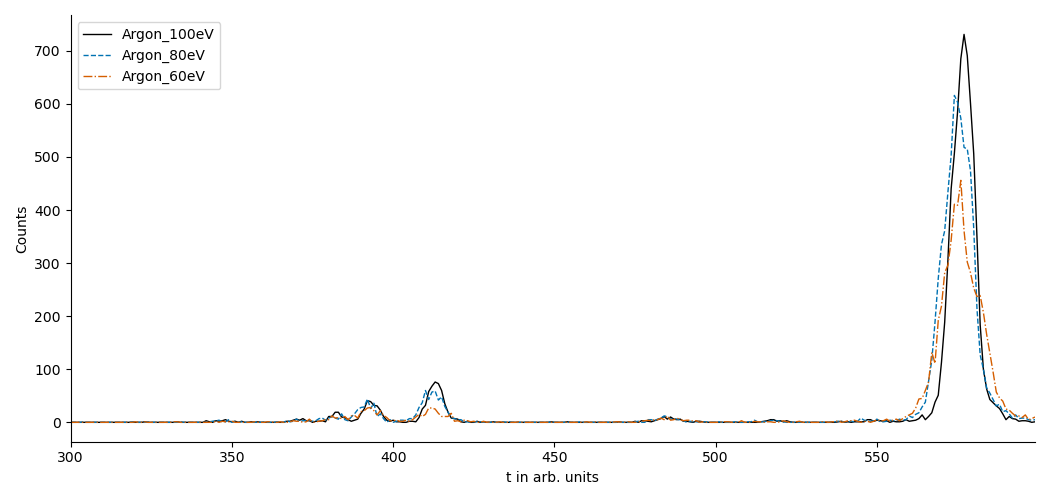
\includegraphics[width=1\textwidth]{Ar60-100.png}
    \caption[Flugzeitspektrum von Argon bei Elektronenenergie 60, 80 und 100 eV]{Flugzeitspektrum von Argon bei Elektronenenergien von 60, 80 und 100 eV. Die Messungen sind jeweils über 60 Sekunden entstanden.}
    \label{fig:ar}
\end{figure}

Abbildung \ref{fig:ar} zeigt ein unskaliertes Flugzeitspektrum von Argon bei verschiedenen Energien. Es ist zu erkennen, dass die Peaks mit steigender Elektronenenergie schärfer werden und es einen Zusammenhang zwischen der Elektronenenergie und der Flugzeit gibt. Woher genau dieser Zusammenhang kommt, kann nicht aus den Daten abgeleitet werden, da ein höherer Energieübertrag auf die Gasatome nicht direkt die Flugzeit beeinflussen kann. Es kann aber vermutet werden, dass dieses Phänomen mit der verzögerten Extraktion der Ionen aus dem Kondensator zusammenhängt, die Ionen mit höheren kintischen Energien schneller beschleunigt. Genauere Untersuchungen folgen im Kapitel \ref{chap:Simulation} zur Simulation. Anhand der mittleren Flugzeit des größten Peaks der verschiedenen Spektren kann der Zusammenhang zwischen der Elektronenenergie und der Flugzeit untersucht werden.
Abbildung \ref{fig:tof_energy} zeigt die Flugzeit des größten Peaks in Abhängigkeit der Elektronenenergie. Es ist zu erkennen, dass die Flugzeit mit steigender Elektronenenergie sinkt. Ein Fit der Form $t = a\sqrt{E} + b$ zeigt, dass die Flugzeit propotional zu $\sqrt{E}$ ist.

\begin{figure}
    \centering
    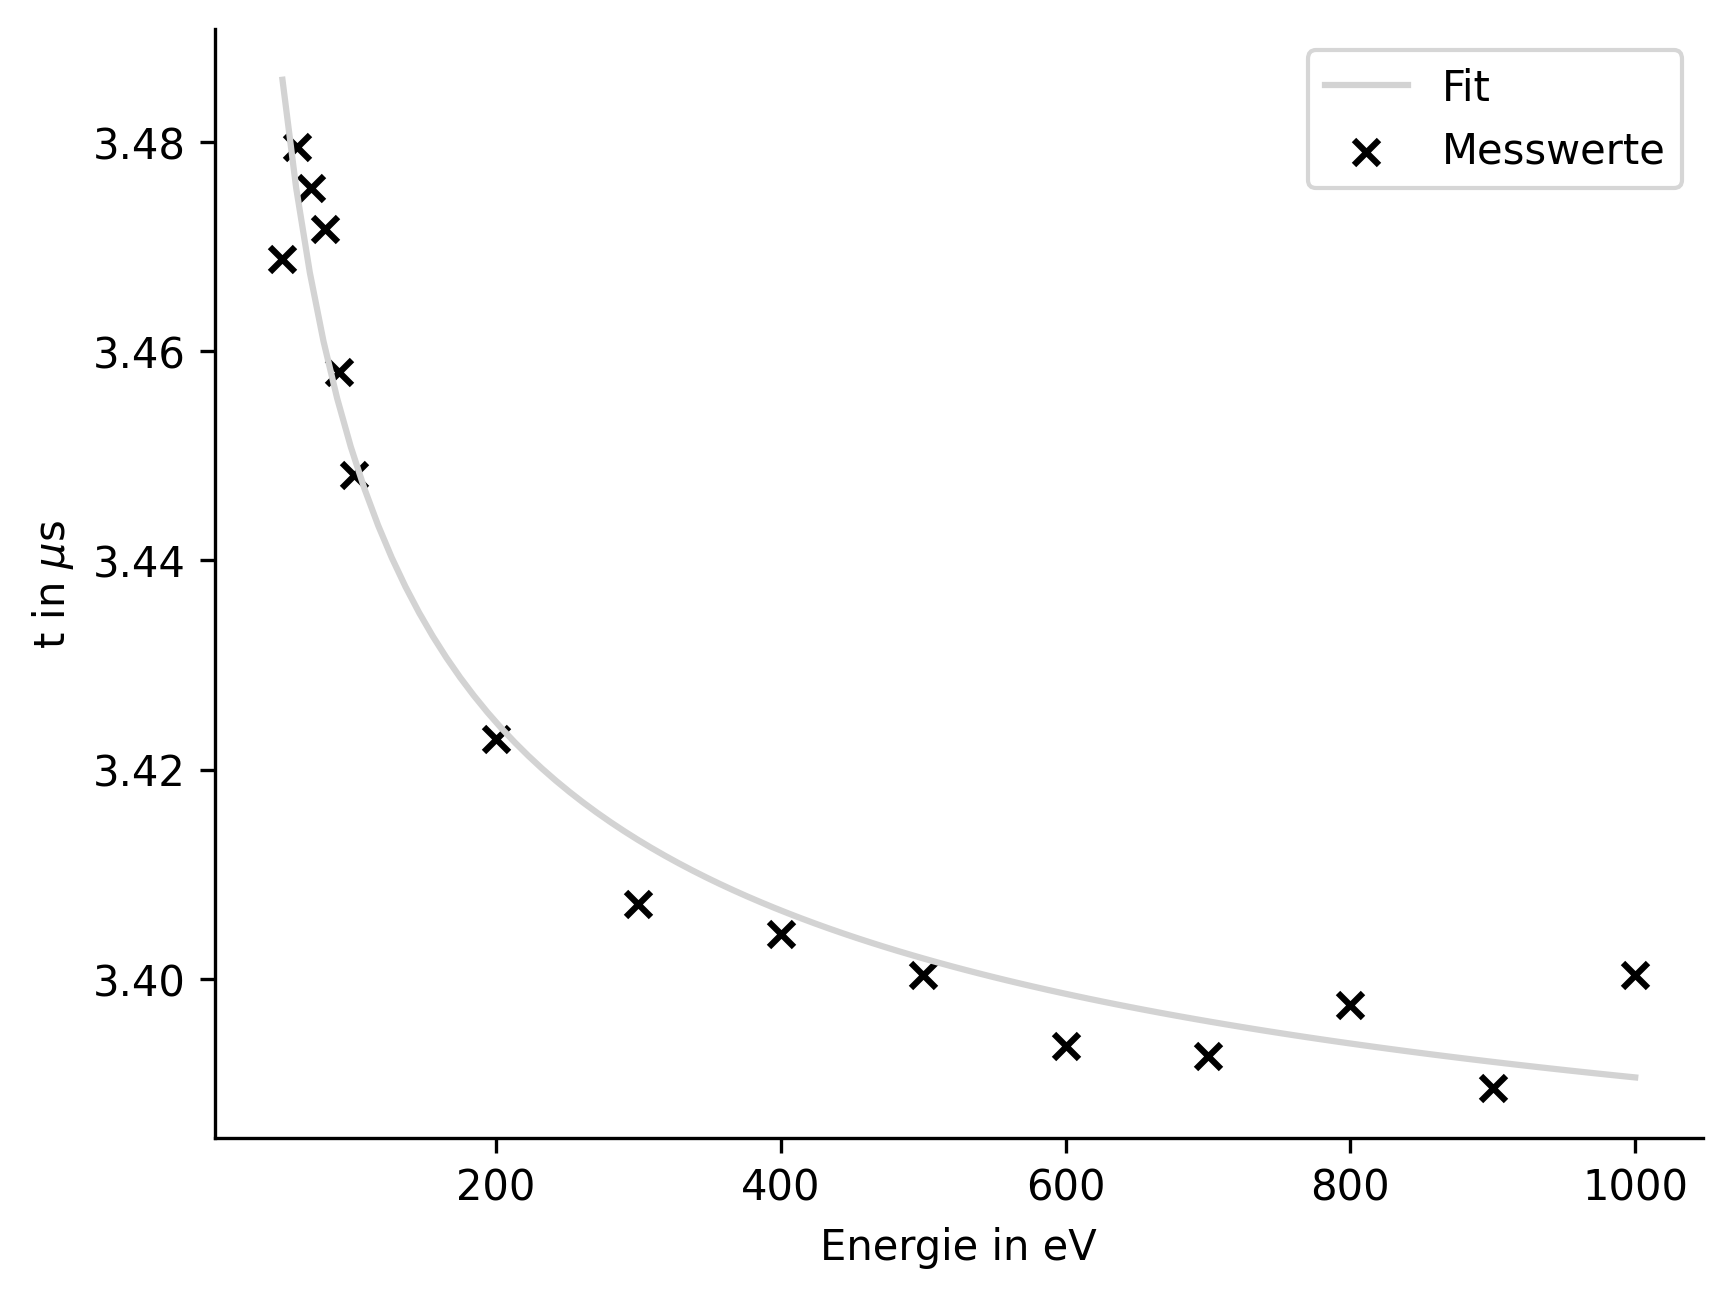
\includegraphics[width=.7\textwidth]{tof_energy.png}
    \caption[Abbildung TOF über Elektronenenergie]{Abbildung der Flugzeit des größten Peaks in Abhängigkeit der Elektronenenergie. Ein Fit zeigt, dass eine Wurzelfunktion die Daten annähert.}
    \label{fig:tof_energy}
\end{figure}

\subsection{Transformation in ein Massenspektrum}
Für eine weitere Analyse muss das Flugzeitspektrum in ein Massenspektrum transformiert werden. Diese Transformation ist nicht linear, da die Flugzeit propotional zu $\sqrt{m/q}$ ist. Um das Spektrum korrekt skalieren zu können, werden die Peaks mit einem Referenzspektrum verglichen und einzelne identifiziert. Im Fall der Kalibrationsmessung mit Argon wurde ein Spektrum von Straub \textit{et al.} \cite{Straub} als Vergleich verwendet, bei dem die Peaks von ein- bis vierfach geladenen Argonionen identifiziert wurden. Anhand dieser Information kann das Spektrum skaliert werden, um die Masse-zu-Ladungsverhältnisse auf der horizontalen Achse zu erhalten. Die Transformationsfunktion hat die Form $a\sqrt{t}+bt+c$, wobei die Parameter über die Zuordnung des Masse-zu-Ladungsverhältnisses von mindestens drei Punkten ermittelt werden können. 

Um einen Vergleich mehrerer Spektren zu ermöglichen, werden die Spektren zunächst normalisiert. Das bedeutet, dass die Fläche des größten Peaks (Ar$^+$) auf 1 gesetzt wird. Da sich der Ionisationsquerschnitt mit der Elektronenenergie ändert, werden die Spektren anschließend mit den Werten für $\sigma^+$ gewichtet. Der Count der Ionen geht direkt proportional in den Ionisierungsquerschnitt $\sigma^+$ ein. Tabelle \ref{tab:argon} zeigt einen Auszug der Ionisierungsquerschnitte von Argon aus \cite{Straub}.

\subsection{Analyse und Vergleich der Ergebnisse}
Abbildung \ref{fig:ar_scaled} zeigt das Spektrum aus Abbildung \ref{fig:ar} nach Anwendung der Transformationsfunktion und Normalisierung. Die Peaks der ein- bis vierfach geladenen Argonionen sind in den Spektren gut zu erkennen. Außerdem sind einige weitere Peaks mit Fragmenten von Wasser, Kohlenstoff und atmosphärischen Gasen sichtbar. Diese werden im nächsten Abschnitt besprochen. Die Spektren zeigen auch, dass erst beim Erreichen einer bestimmten Elektronennergie Mehrfachionisationprozesse stattfinden können. Die Wirkungsquerschnitte für die Mehrfachionisationen sind zwar deutlich kleiner als für die DI, dennoch nimmt der Anteil der DI als Folge mit steigender Elektronenerngie ab. Dass dieser Effekt sichtbar ist, zeigt, dass die Ionisation in der Anlage erfolgreich unter Einzelstoßbedingungen stattfindet.

\begin{landscape}
    \begin{figure}
        \centering
        \hspace*{-3cm}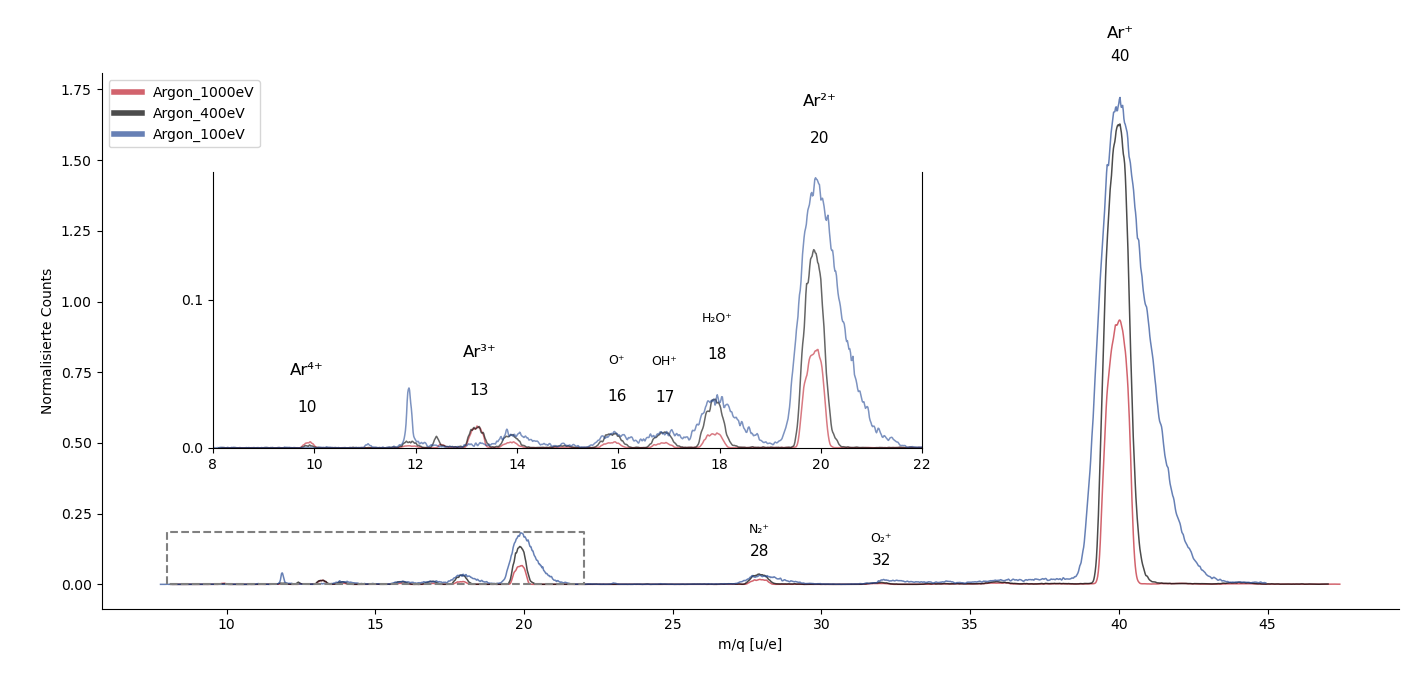
\includegraphics[width=1.7\textwidth]{Ar_scaled.png}
        \caption[Skaliertes Massenspektrum von Argon bei verschiedenen Elektronenenergie]{Masse-zu-Ladungsspektrum von Argon bei Elektronenenergien von 100, 400 und 1000 eV. Die Messungen sind jeweils über 30 Minuten entstanden. Die Spektren wurden normarlisiert und sind mit den Werten aus \ref{tab:argon} gewichtet dargestellt. Außerdem wurden sie mit einem gauß'schen 1D-Filter ($\sigma = 1$) leicht geglättet, um sie besser vergleichen zu können.}
        \label{fig:ar_scaled}
    \end{figure}
\end{landscape}

Obwohl die Werte für die Ionisierungsquerschnitte aufgrund der defekten Kanone nicht direkt ermittelt werden können, soll anhand der relativen Häufigkeiten der Ionen eine qualitative Aussage über die relativen Ionisierungsquerschnitte getroffen werden. Das bedeutet, dass das Verhältnis $\sigma^+$/$\sigma^{2+}$ dem Verhältnis der Flächen $A(\text{Ar}^+)$/$A(\text{Ar}^{2+})$ entsprechen sollte. Dies kann mit einem direkten Vergleich  mit den Werten aus \ref{tab:argon} überprüft werden. Abbildung \ref{fig:ar_ratio} zeigt die Grenzen der Integration und die Bestimmung der Verhältnisse. Für einen einfachen Vergleich wurde die Fläche des Ar$^+$-Peaks auf 0.795 gesetzt, dem entsprechenden Quersschnitt aus Tab. \ref{tab:argon}. In Tabelle \ref{tab:vergleich} sind die normierten Werte der Ionen und die prozentualen Abweichungen zu den Werten von Straub \textit{et al.} \cite{Straub} angegeben. Es ist zu erkennen, dass die Werte für die ein- und zweifach geladenen Ionen besser übereinstimmen, während die Werte für die dreifach und vierfach geladenen Ionen größere prozentuale Abweichungen haben. Dies ist vermutlich auf die geringe Anzahl an Ionen zurückzuführen, die bei höheren Energien entstehen. Insgesamt zeigt die qualitative Auswertung, dass die Anlage erfolgreich arbeitet, da die relativen Häufigkeiten der Ionen den Erwartungen in etwa entsprechen. 

Beim Summieren der einzelnen Querschnitte zum totalen Querschnitt werden die Werte entsprechend der Ladung gewichtet:
\begin{equation}
    \sigma^{\text{total}} = \sigma^+ + 2\sigma^{2+} + 3\sigma^{3+} + 4\sigma^{4+}.
\end{equation}
Die Summe der normierten Ionenzahlen Tabelle \ref{tab:vergleich} equivalent berechnet.

\begin{figure}
    \centering
    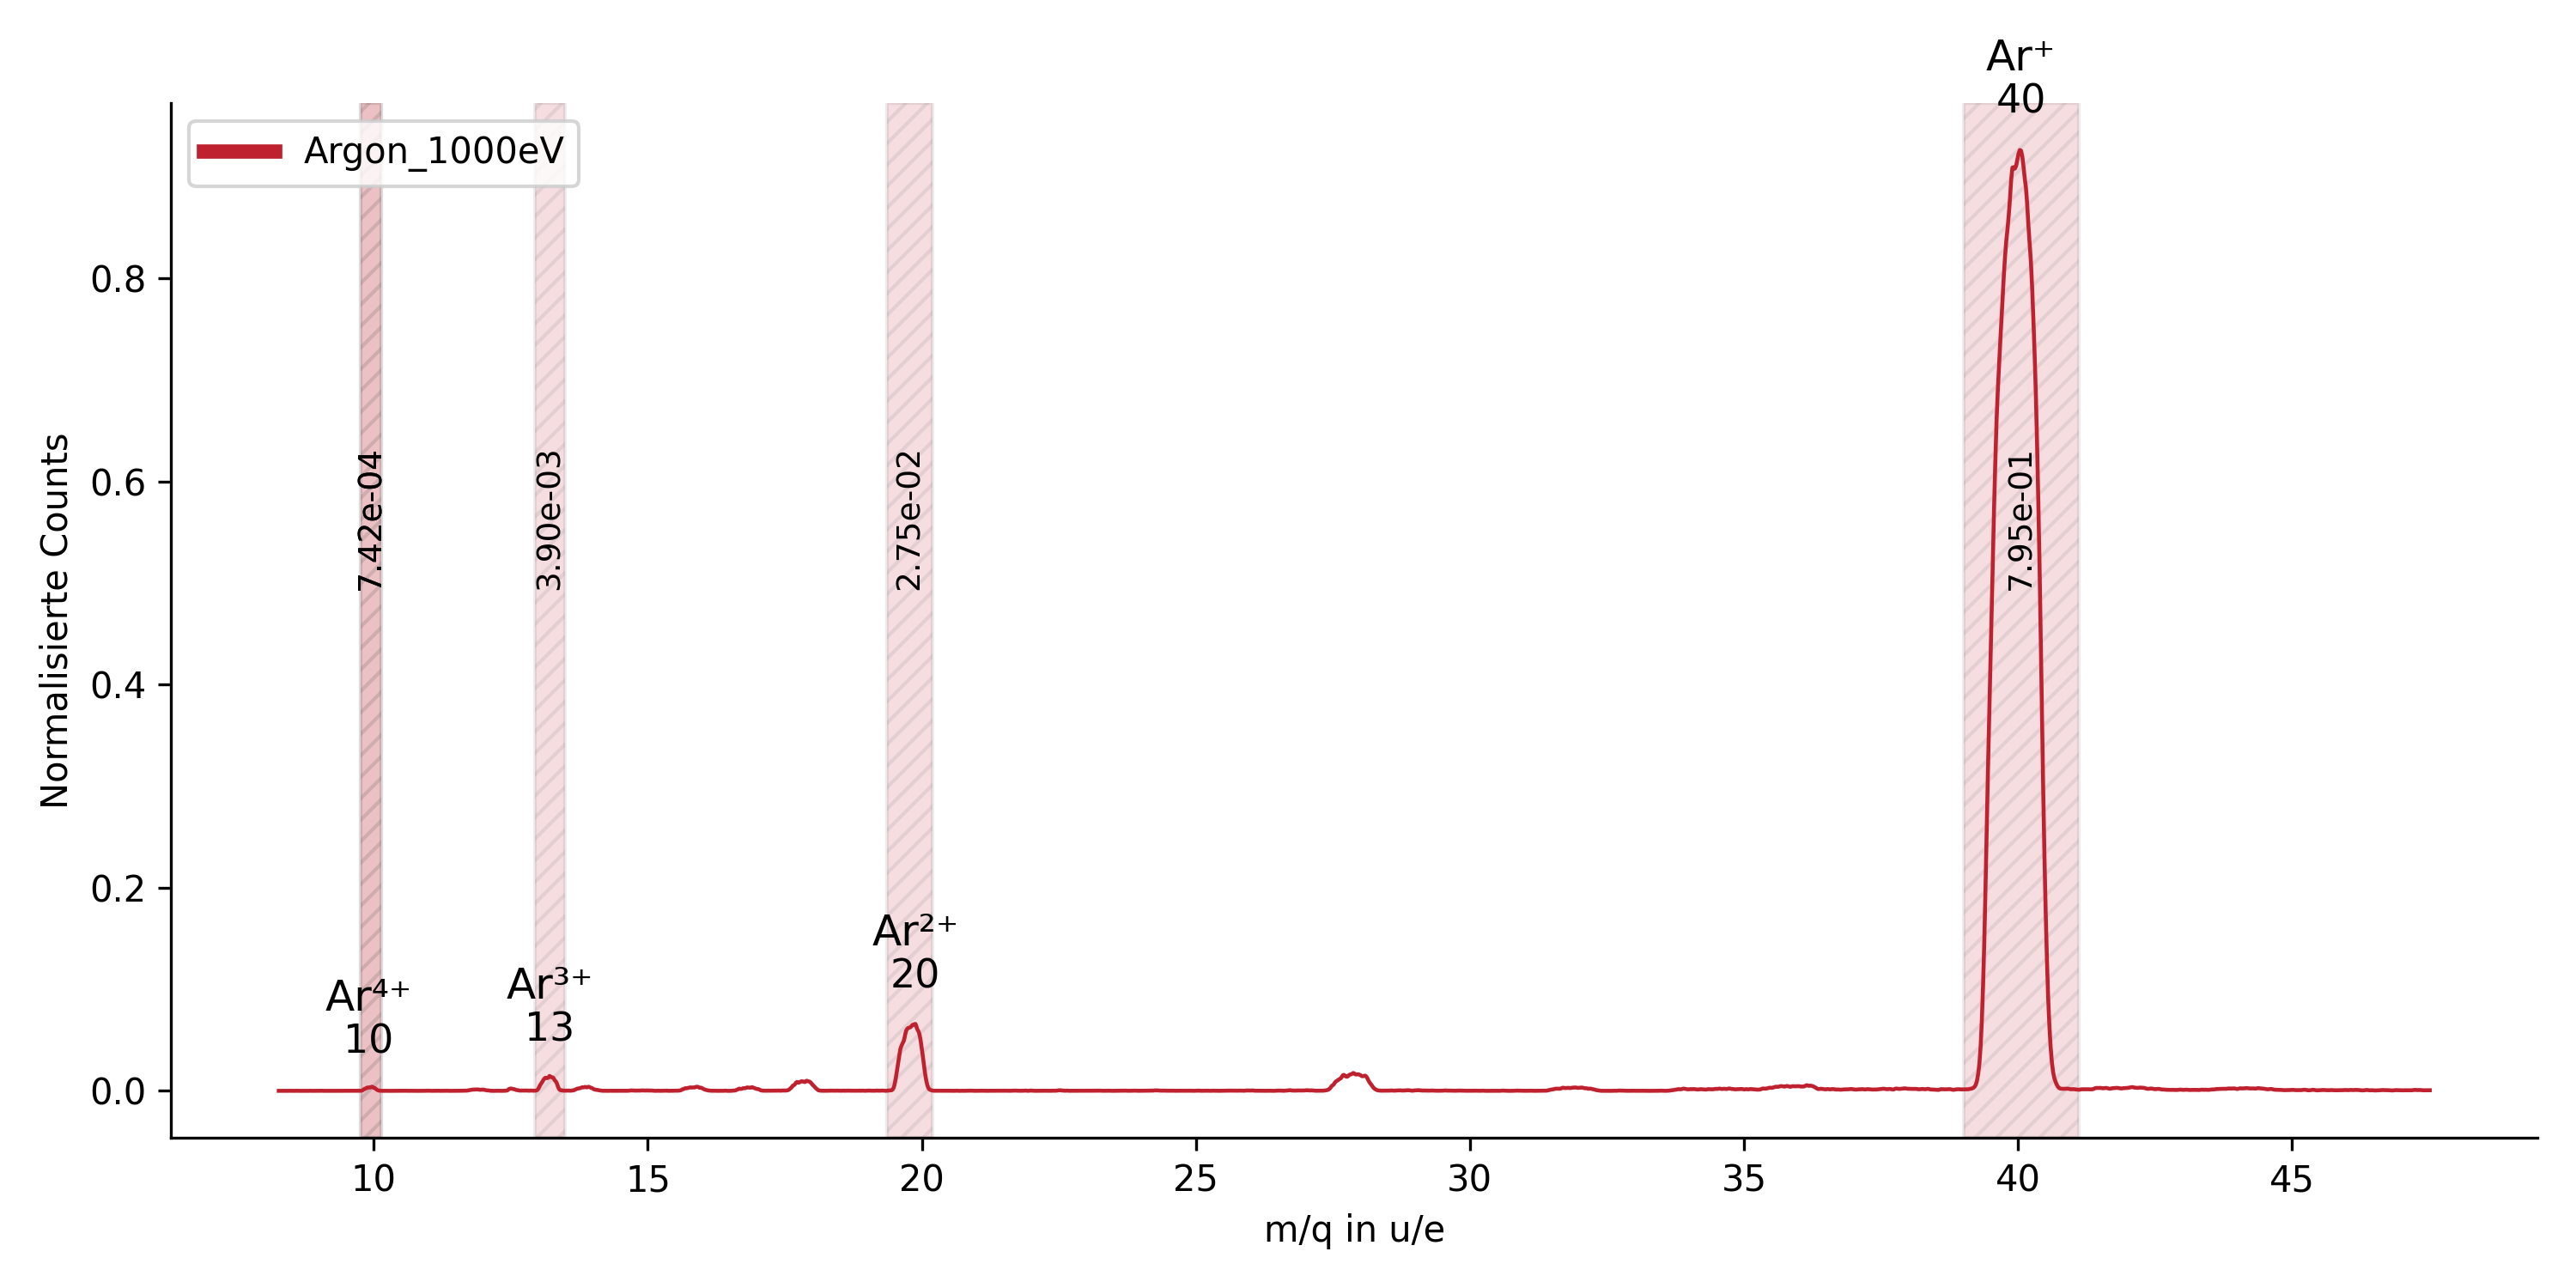
\includegraphics[width=1\textwidth]{Ar_integrated.png}
    \caption[Integration eines gewichteten Argonspektrums bei 1000 eV]{Integration eines gewichteten Argonspektrums bei 1000 eV.}
    \label{fig:ar_ratio}
\end{figure}

\begin{table}
    \centering
    \caption[Auszug der Ionisierungsquerschnitte von Argon aus Straub \textit{et al.} \cite{Straub}]{Auszug der Ionisierungsquerschnitte von Argon aus Straub \textit{et al.} \cite{Straub}}
    \label{tab:argon}
    \begin{tabular}{r c c c c c}
        \toprule
        \textbf{Energie} & $\sigma^+$ & $\sigma^{2+}$ & $\sigma^{3+}$ & $\sigma^{4+}$ & $\sigma^{\text{total}}$ \\
        (eV) & ($10^{-16}$ cm$^2$) & ($10^{-17}$ cm$^2$) & ($10^{-19}$ cm$^2$) & ($10^{-19}$ cm$^2$) & ($10^{-16}$ cm$^2$) \\
        \midrule
        %17  & 0.017  &        &        &        & 0.017  \\
        %20  & 0.46   &        &        &        & 0.46   \\
        %25  & 1.24   &        &        &        & 1.24   \\
        %30  & 1.84   &        &        &        & 1.84   \\
        %35  & 2.26   &        &        &        & 2.26   \\
        %40  & 2.55   &        &        &        & 2.55   \\
        %45  & 2.66   & 0.0048 &        &        & 2.66   \\
        50  & 2.70   & 0.128  &        &        & 2.73   \\
        %55  & 2.69   & 0.418  &        &        & 2.77   \\
        %60  & 2.67   & 0.856  &        &        & 2.84   \\
        %65  & 2.67   & 1.21   &        &        & 2.91   \\
        %70  & 2.67   & 1.46   &        &        & 2.96   \\
        %75  & 2.66   & 1.56   &        &        & 2.97   \\
        %80  & 2.69   & 1.70   &        &        & 3.03   \\
        %85  & 2.70   & 1.79   &        &        & 3.06   \\
        %90  & 2.69   & 1.84   &        &        & 3.06   \\
        %95  & 2.67   & 1.90   & 0.51   &        & 3.05   \\
        100 & 2.64   & 1.89   & 1.03   &        & 3.02   \\
        %110 & 2.61   & 1.91   & 2.21   &        & 3.00   \\
        %120 & 2.55   & 1.87   & 3.23   &        & 2.93   \\
        %140 & 2.45   & 1.77   & 4.94   &        & 2.81   \\
        %160 & 2.35   & 1.65   & 5.57   &        & 2.70   \\
        %180 & 2.27   & 1.58   & 5.68   &        & 2.60   \\
        %200 & 2.18   & 1.44   & 5.53   &        & 2.49   \\
        %225 & 2.10   & 1.31   & 5.30   &        & 2.37   \\
        %250 & 1.99   & 1.25   & 5.23   &        & 2.25   \\
        %275 & 1.87   & 1.13   & 5.09   &        & 2.11   \\
        %300 & 1.79   & 1.08   & 5.03   &        & 2.02   \\
        %350 & 1.63   & 0.953  & 5.99   & 0.17   & 1.84   \\
        400 & 1.51   & 0.872  & 6.32   & 0.44   & 1.71   \\
        %450 & 1.39   & 0.759  & 6.50   & 0.77   & 1.57   \\
        %500 & 1.31   & 0.679  & 6.97   & 1.07   & 1.47   \\
        %550 & 1.23   & 0.623  & 7.08   & 1.18   & 1.38   \\
        %600 & 1.16   & 0.575  & 7.41   & 1.32   & 1.30   \\
        %650 & 1.09   & 0.552  & 7.19   & 1.27   & 1.23   \\
        %700 & 1.03   & 0.524  & 7.23   & 1.33   & 1.16   \\
        %750 & 0.976  & 0.496  & 6.97   & 1.42   & 1.10   \\
        %800 & 0.932  & 0.456  & 6.96   & 1.50   & 1.05   \\
        %850 & 0.901  & 0.425  & 7.09   & 1.42   & 1.01   \\
        %900 & 0.865  & 0.419  & 6.51   & 1.33   & 0.973  \\
        %950 & 0.824  & 0.394  & 6.51   & 1.36   & 0.927  \\
        1000 & 0.795 & 0.374  & 6.57   & 1.32   & 0.895  \\
        \bottomrule
    \end{tabular}
\end{table}


\begin{table}
    \centering
    \caption[Normierte Anzahl von Ionen und Abweichung zu Werten von Straub \textit{et al.}]{Normierte Anzahl von Ionen dargestellt wie in Tab. \ref{tab:argon}. In Klammern sind die prozentualen Abweichungen zu den Werten von Straub \textit{et al.} \cite{Straub} angegeben.}
    \label{tab:vergleich}
    \begin{tabular}{r c c c c c}
        \toprule
        \text{} & \multicolumn{5}{c}{\textbf{normierte Anzahl von Ionen}} \\ 

        \textbf{Energie} & $Ar^+$ & $Ar^{2+}$ & $Ar^{3+}$ & $Ar^{4+}$ & gew. Summe \\
        (eV) & (1) & ($10^{-1}$) & ($10^{-3}$) & ($10^{-3}$) & ($1$) \\
        \midrule
        50  & {TODO}  & {TODO}  & {}  & {}  & {TODO}   \\
        100 & 2.64  & 1.42 \textcolor{gray}{(24.9\ \%)} & 4.04 \textcolor{gray}{(292.2\ \%)} & {} & 2.94 \textcolor{gray}{(7.1\ \%)} \\
        400 & 1.51  & 0.602 \textcolor{gray}{(31.0\ \%)} & 4.62 \textcolor{gray}{(26.9\ \%)} & 0 \textcolor{gray}{(100\ \%)} & 1.64 \textcolor{gray}{(4.3\ \%)} \\
        1000 & 0.795  & 0.278 \textcolor{gray}{(25.7\ \%)} & 3.98 \textcolor{gray}{(39.4\ \%)} & 0.763 \textcolor{gray}{(42.2\ \%)} & 0.86 \textcolor{gray}{(4.1\ \%)} \\
               
        
        \bottomrule
    \end{tabular}
\end{table}

\section{Restgasspektrum}
Eine weitere Möglichkeit zur Überprüfung des Massenspektrometers ist die Aufnahme eines Restgasspektrums. Hierbei wird kein Gas in die Kammer eingelassen und lediglich der atmosphärische Hintergrund in der Kammer gemessen. Dieser besteht aus verschiedenen Restgasen, die durch die Elektronenstoßionisation genauso ionisiert werden können. In einem Vakuum erwartet man vorallem Rückstände von Wassermolekülen, sowie stabiler Kohlenstoffverbindungen, die bei der Vakuumbildung aus den Wänden der Kammer gelöst werden, als auch Reste von Stickstoff und Sauerstoff aus der Luft. Außerdem können besonders leichte Gase, hier vorallem Wasserstoff, übrig bleiben, da sie besonders flüchtig sind und die Vakuumpumpen sie weniger effektiv entfernen können. Es ist zusätzlich praktisch die Restgasverteilung zu kennen, um sie bei der Auswertung von Messungen berücksichtigen zu können. Aufgrund der geringen Dichte und damit niedrigem Ionisierungsquerschnitt muss diese Messung lange durchgeführt werden. 

Wie bereits bei der Kalibrationsmessung muss das Massespektrum transformiert werden, um die Masse-zu-Ladungsverhältnisse der Ionen zu bestimmen. Dafür wird für einige der Peaks anhand von den Erwartungen eine Annahme getroffen, welchem Verhältnis sie entsprechen könnten. Für die Identifikation der Ionen wurde angenommen, das der größte Peak ionisierten Wassermolekülen
entspricht und der erste Peak ionisiertem Wasserstoff. Das resultierende, skalierte Restgasspektrum ist in Abb. \ref{fig:rest} dargestellt.

Wie erwartet können die größten Peaks auf ionisierte Wassermoleküle, sowie Wasserstoff zurückgeführt werden. Auch die Peaks von molekularem Stickstoff, Sauerstoff und vermutlich Kohlenstoffdioxid sind gut zu erkennen. Die Struktur und Übereinstimmung des Restgasspektrums zeigen, dass die Anlage korrekt funktioniert und zur Identifikation von Produktionen taugt. Außerdem ist zu erkennen, dass Massendifferenzen von 1 $u$ im Bereich leichter Ionen aufgelöst werden können. 

\begin{figure}
    \centering
    \hspace*{-1cm}
    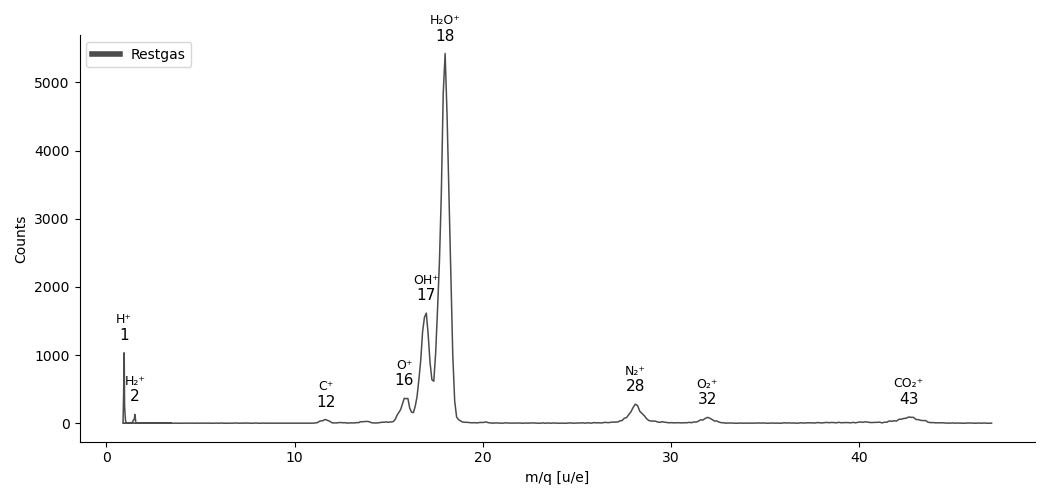
\includegraphics[width=1.05\textwidth]{Restgas.png}
    \caption[Masse-zu-Ladungsspektrum der Restgase]{Masse-zu-Ladungsspektrum der Restgase erzeugt aus dem Flugzeitspektrum in Abb. \ref{fig:rest_tof}. Die Peaks entsprechen den verschiedenen Ionen, die durch die Elektronenstoßionisation entstanden sind. Das Spektrum wurde skaliert, um die Masse zu Ladungsverhältnisse der Ionen zu bestimmen.}
    \label{fig:rest}
\end{figure}

\section{Auswertung der Positionsdaten}
Anhand der vom Detektor aufgenommenen Positionsdaten der Ionen, können Rückschlüsse auf den Entstehungsort der Ionen gezogen werden. Abbildung \ref{fig:Strahl} zeigt einen Plot dieser Daten für eine Messung mit Argonionen. Es ist zu erkennen, dass die Ionen, wie erwartet, entlang eines horizontalen Streifens entstehen, der seitlich abgeschnitten ist. Die Ionen wurden durch das 2 cm große Loch in der Deckenplatte des Beschleunigungskondesators auf den Detektor geschossen. Deshalb ist das Abbild des Elektronenstrahls seitlich begrenzt. Die Entstehungsorte der Ionen sind offensichtlich stark mit dem Strahl verbunden, was zeigt, dass die Ionen entlang des Strahls entstehen und nicht wesentlich abgelenkt werden oder aus anderen Quellen stammen.

\subsection{Annomalien}
Auffällig sind jedoch die Überhöhungen an den seitlichen Rändern des Strahls, die in Abbildung \ref{fig:Strahl3D} besonders deutlich zu erkennen sind. Außerdem ist die Länge des Abbilds von 28 mm unvorhergesehen. Bei geraden Flugbahnen der Ionen würde ein Abbild von etwa 20 mm Länge erwartet werden, entsprechend dem Loch in der Deckenplatte. Anders als bei einem Ionenstrahl, bei dem die Coloumbabstoßung eine Aufweitung bewirkt, sollte kein solcher Effekt unter der Einzelstoßbedingung auftreten. Beide dieser Effekte sollen mit der Simulation der Ionenoptik überprüft werden, um eine mögliche Erklärung zu finden. Die leichte Wölbung des Strahls war während des Experiments konstant und kann nur auf eine Ungenauigkeit der vom Detektor ermittelten Positionen zurückgeführt werden. 
\begin{figure}
    \centering
    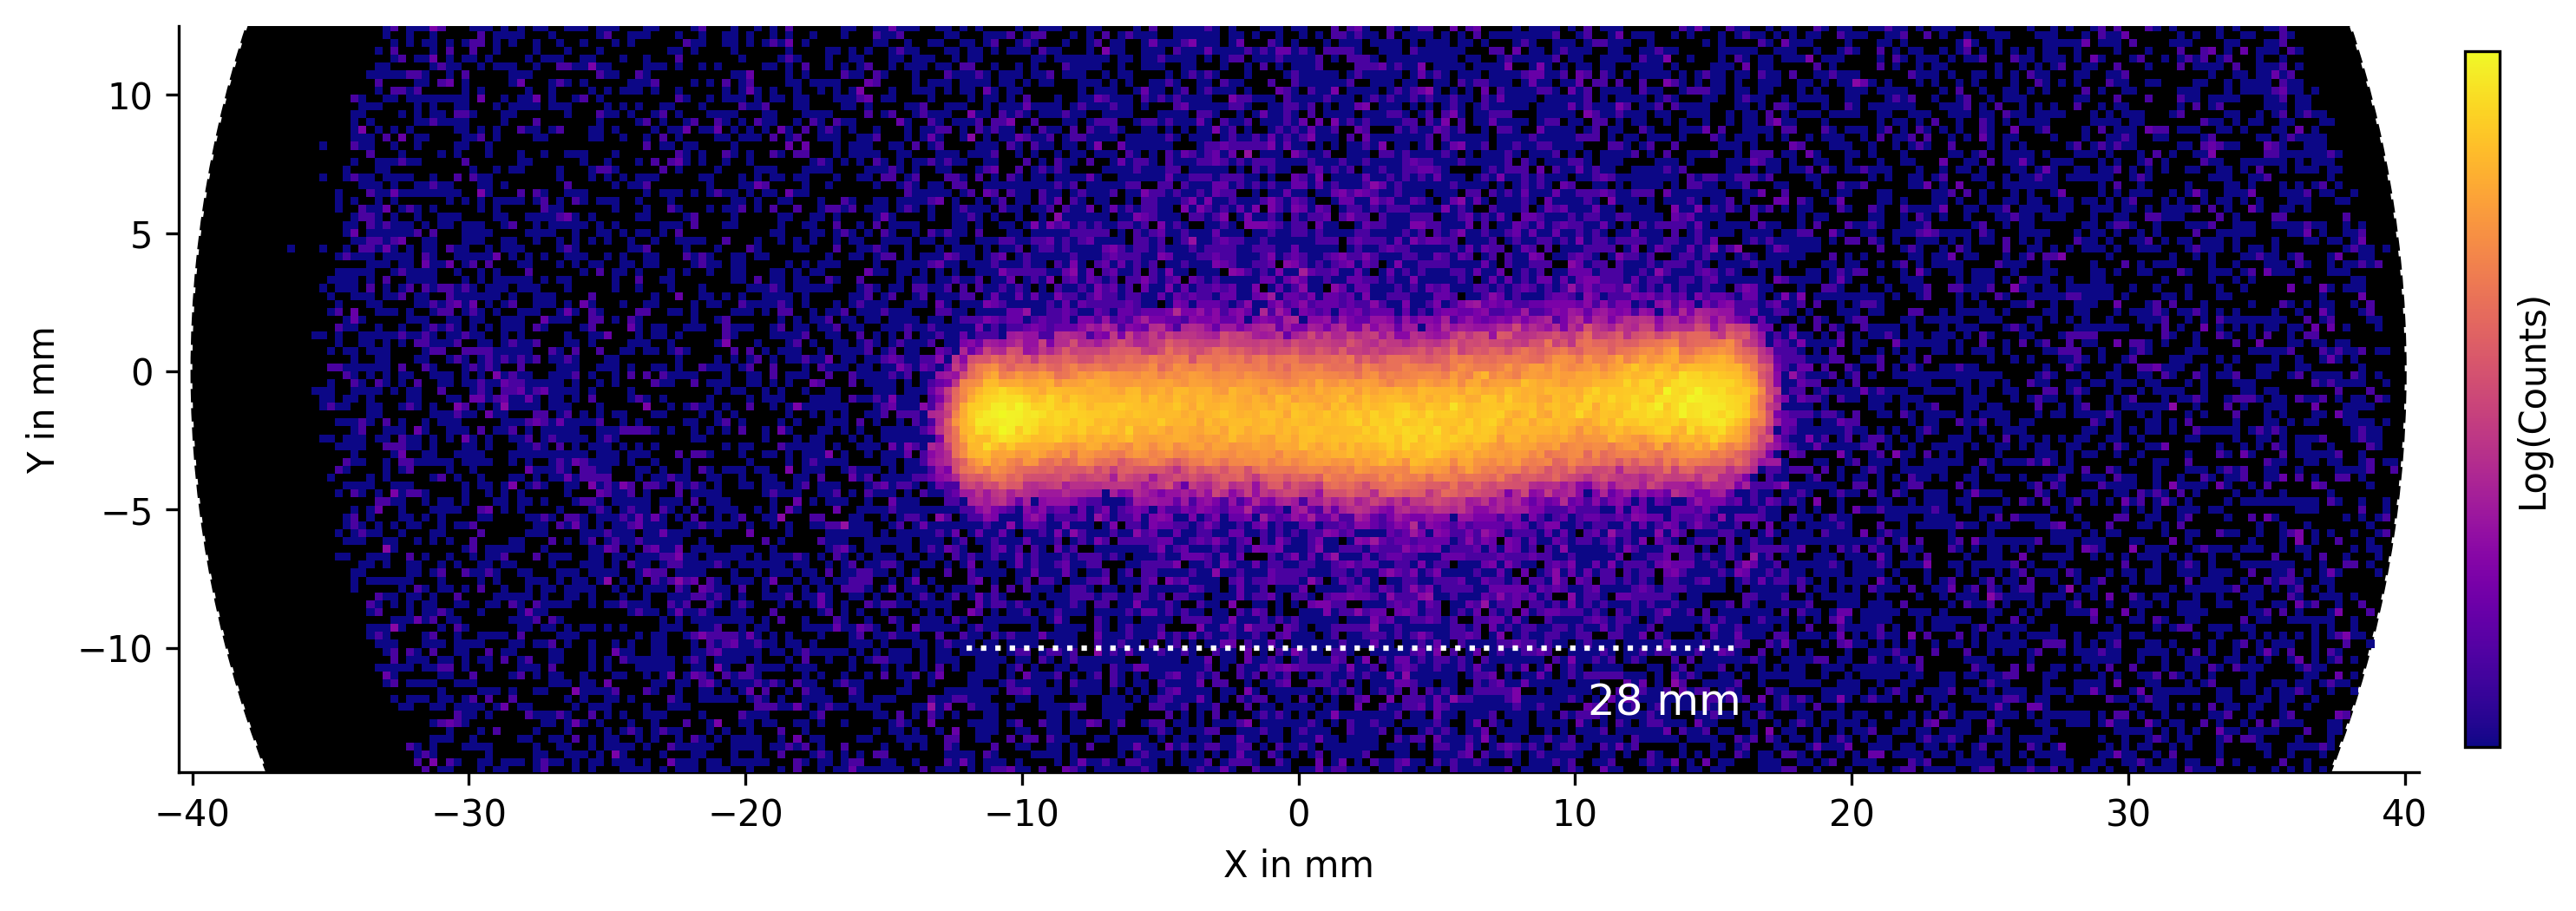
\includegraphics[width=1.05\textwidth]{Strahl.png}
    \caption[Logaritmisches Abbild des Strahls auf dem Detektor]{Positionsbestimmung der detektierten Teilche auf dem Detektor zeigen den Strahl auf dem Detektor. Die Anzahl der Treffer in einem Pixel wird logarithmisch skaliert von den Farben angegeben. Da der Detektor schief verbaut ist, wurde das Bild im Nachhinein gedreht. Das Abbild des Strahls ist seitlich begrenzt, da die Ionen durch das 2 cm große Loch in der Deckenplatte auf den Detektor gelangen. Die geometrische Größe des Detektors ist in Schwarz eingezeichnet.}
    \label{fig:Strahl} 
\end{figure}

\begin{figure}
    \centering
    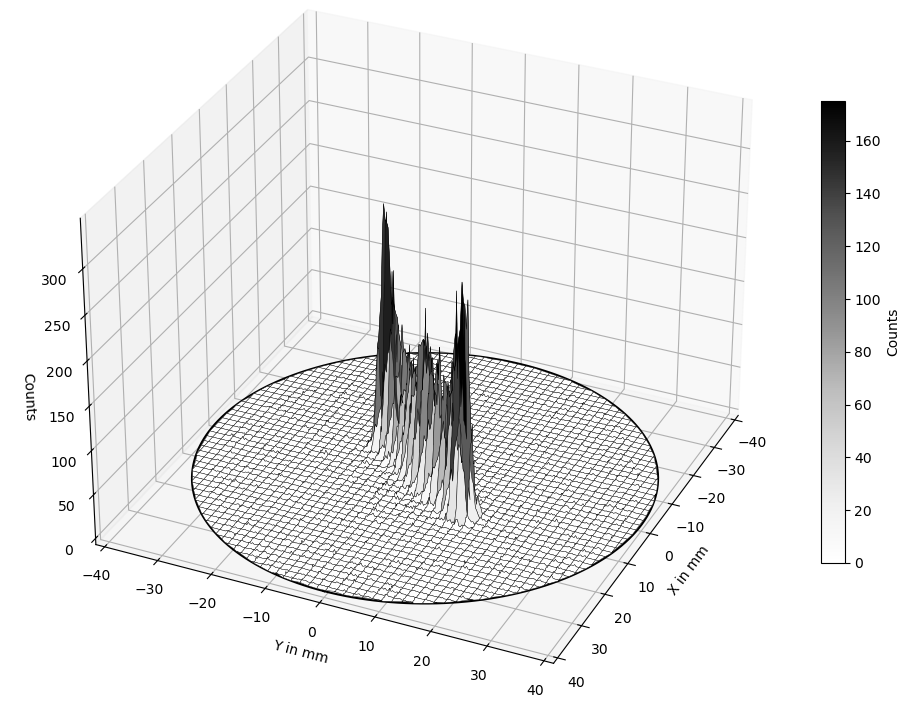
\includegraphics[width=.85\textwidth]{Strahl3D.png}
    \caption[Dreidimensionales Abbild des Strahls auf dem Detektor]{Dreidimensionales Abbild des Strahls auf dem Detektor. Die Anzahl der Treffer ist absolut dargestellt. Die Überhöhungen an den Rändern des Strahls sind gut zu erkennenbar. Das Bild zeigt die tatsächliche Ausrichtung des Detektors relativ zum Strahl.}
    \label{fig:Strahl3D} 
\end{figure}

\subsection{Ermittlung des Elektronenstrahlprofil}
Die Positionen der detektierten Ionen auf dem Detektor können genutzt werden, um das Strahlprofil, also die räumliche Verteilung der Teilchen in einem Schnitt des Strahls, zu bestimmen. Um das Strahlprofil über die ganze abgebildete Länge zu mitteln, wird Daten-Binning genutzt. Das bedeutet, dass für jede y-Koordinate in einem \textit{Bin} die Counts aller detektierten Ionen aufsummiert werden. Das Ergebnis ist ein Histogramm, das die räumliche Verteilung der Elektronen entlange der y-Achse zeigt. Das Ergebnis ist in Abb. \ref{fig:Strahlprofil} dargestellt. Für das Profil des Strahls wird eine Gauß-Verteilung erwartet, da thermische Effekte und Beugung die Position der Elektronen zufällig beeinflussen. Mit einem Fit der Daten mit einer Gauß-Funktion kann die Breite des Strahls bestimmt werden. In der Abbildung ist zu erkennen, dass die Abweichung der Daten vom Fit sehr klein ist. Über die Parameter der gefitteten Funktion kann die volle Breite bei halbem Maximum (FWHM) des Strahls bestimmt werden. Sie beträgt 2.93 mm. Obwohl diese Strahlbreite in die vom Hersteller angegebene Fleckgröße von 5 mm passt, ist sie wahrscheinlich, ähnlich wie die horizontale Länge des Strahls, tatsächlich kleiner. Wenn man annimmt, dass die Vergrößerung entlang der y-Achse ähnlich der entlang der x-Achse ist, sollte der Strahl eine FWHM von etwa 2 mm aufweisen.

\begin{figure}
    \centering
    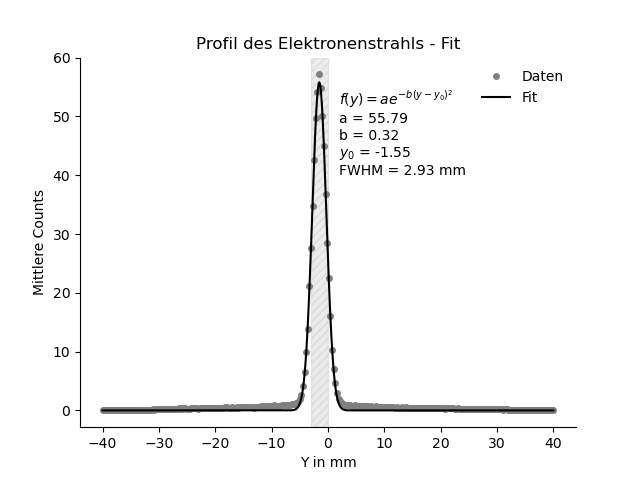
\includegraphics[width=.7\textwidth]{Strahlprofil.png}
    \caption[Gemitteltes Strahlprofil]{Gemitteltes Strahlprofil aus den Positionen der detektierten Ionen. Die Daten wurden mit einem Gaußfit gefittet, um die Breite des Strahls zu bestimmen. In grau-schraffiert eingezeichnet ist die volle Breite bei halbem Maximum (FWHM) des Strahls abgebildet.}
    \label{fig:Strahlprofil} 
\end{figure}